\documentclass[11pt]{article}
\usepackage{geometry}                
\geometry{letterpaper}                   

\usepackage{listings}
\usepackage{graphicx}
\usepackage{amssymb}
\usepackage{epstopdf}
\usepackage[numbers]{natbib}
\usepackage{amssymb, amsmath}
\DeclareGraphicsRule{.tif}{png}{.png}{`convert #1 `dirname #1`/`basename #1 .tif`.png}

\title{Modelling Situations of Evacuation in a Multi-level Building}
\author{Hans Hardmeier, Andrin Jenal, Beat Küng & Felix Thaler}
\date{date} 

\begin{document}



\thispagestyle{empty}

\begin{center}

\includegraphics[width=5cm]{ETHlogo.eps}

\bigskip


\bigskip


\bigskip


\LARGE{ 	Lecture with Computer Exercises:\\ }
\LARGE{ Modelling and Simulating Social Systems with MATLAB\\}

\bigskip

\bigskip

\small{Project Report}\\

\bigskip

\bigskip

\bigskip

\bigskip


\begin{tabular}{|c|}
\hline
\\
\textbf{\LARGE{Insert Title Here}}\\
\textbf{\LARGE{...}}\\
\\
\hline
\end{tabular}
\bigskip

\bigskip

\bigskip

\LARGE{Name 1 \& Name 2}



\bigskip

\bigskip

\bigskip

\bigskip

\bigskip

\bigskip

\bigskip

\bigskip

Zurich\\
March 2012\\

\end{center}



\newpage

%%%%%%%%%%%%%%%%%%%%%%%%%%%%%%%%%%%%%%%%%%%%%%%%%

\newpage
\section*{Agreement for free-download}
\bigskip


\bigskip


\large We hereby agree to make our source code for this project freely available for download from the web pages of the SOMS chair. Furthermore, we assure that all source code is written by ourselves and is not violating any copyright restrictions.

\begin{center}

\bigskip
\bigskip
\bigskip
\bigskip


\begin{tabular}{@{}p{3.3cm}@{}p{6cm}@{}@{}p{6cm}@{}}

\begin{minipage}{3cm}

\end{minipage}
&
\begin{minipage}{6cm}
\vspace{2mm} \large Hans Hardmeier

 \vspace{\baselineskip}

\end{minipage}
&
\begin{minipage}{6cm}

\large Andrin Jenal

\end{minipage}

\end{tabular}

\bigskip
\bigskip
\bigskip
\bigskip


\begin{tabular}{@{}p{3.3cm}@{}p{6cm}@{}@{}p{6cm}@{}}

\begin{minipage}{3cm}

\end{minipage}
&
\begin{minipage}{6cm}
\vspace{2mm} \large Beat Küng

 \vspace{\baselineskip}

\end{minipage}
&
\begin{minipage}{6cm}

\large Felix Thaler

\end{minipage}
\end{tabular}

\end{center}
\newpage

%%%%%%%%%%%%%%%%%%%%%%%%%%%%%%%%%%%%%%%



% IMPORTANT
% you MUST include the ETH declaration of originality here; it is available for download on the course website or at http://www.ethz.ch/faculty/exams/plagiarism/index_EN; it can be printed as pdf and should be filled out in handwriting

%TODO: The is declaration of originality on the WEb for Windows (Andrin Jenal)...

%%%%%%%%%% Table of content %%%%%%%%%%%%%%%%%

\tableofcontents

\newpage

%%%%%%%%%%%%%%%%%%%%%%%%%%%%%%%%%%%%%%%



\section{Abstract}

%% TODO: No idea what to write - Summary (Hans Hardmeier End)

\section{Individual contributions}



%TODO: Wer het was gmacht... (Jede : Beat, Hans, Andrin, Felix)

\section{Introduction and Motivations}

\subsection{Introduction}

Simulating the evacuation scenario of a single-level building is well known but is not general enough. Though we want to introduce a more sophisticated simulation within a multi-level building. E.g.: What would happen, if a multi-level building has to be evacuated? Which escape routes would be mostly used? Which effects would have the pressure/panic of other persons into the situation? Since tower buildings are getting more common in large cities, engineers have to care more about the behaviour in situations of emergency, namely evacuations. 

\subsection{Motivation}

Intuitive expectations and mathematical model results can stay sometimes in contradictions. To prove the rational expected results of i.e. evacuation of the ETH, we want to provide a flexible tool that is able to calculate every scenario in every provided structure with certains requirements.

\section{Description of the Model}

%TODO: finalize (write out every etc.) Hans compare with RESEARCH! -> Froge zerscht (Beim Introduction)und ausschreiben
% TODO MERGE WITH RESEARCH!!! Andrin Jenal

To investigate it, we will create a relatively general framework for behavioral simulation in evacuation scenarios. That includes every non-trivial, relevant force affecting every agent i.e. repulsion within the agents (unconscious privacy area conservation), detection of environment (walls, exits, stairs - inclusive direction-, evtl. source of evacuation,etc ) rational thinking to calculate the way to exit (run-time calculation with fast-sweeping algorithm), etc.


\subsection{General Model}

We are planning to base our work on the social force model \cite{SFMPD}. The  behaviour of the agents will be mainly influenced by different model parameters like obstacles, stairs and other agents. In addition, psychological pressure in such evacuation scenarios are going to be investigated. The following points are the chosen parameters for the model in this work. For more precisely mathematical explanations, see \cite{SFMPD}




\subsection*{Agents Repultion Force}

Within a evacuation scenario, the psychological tendency of two pedestrians i and j to stay away from each other, depends on the level of repultion between this two specific agents (margin of unconscious privacy area conservation between them). In addition, we assume two other more physical forces: a `body force' counteracting body compression (important factor in a panic evacuation model) and a `sliding friction force' avoiding the unnatural regulation of the speed when the agent nears another. 

\subsection*{Physical Objects}

Using the nearest point in a wall to an agent, the repulsive forces created by the whole wall is treaten analog as the created Agents-Repultion-Forces. At the same time, the preprocessing of the map, together with the exits and stairs, allows us to create a gradient field all over the map, that shows the agent, the shortest way to exit the floor. 

%%Evtl.  example of field force?? from /images


\subsection*{Force of Agents}

Quote from 'Helbling, Dirk - Molnar, Peter (1995): Social Force Model for Pedestrians Dynamics' \cite{SFMPD} :

\textit{"The desired velocity $v^0_i$ can reach more than $5 ms^{-1}$ (up to $10 m s^{-1}$), but the observed free velocities	for	leaving	a	room	correspond	to	$v^0_i=6 ms^{-1}$ under relaxed, $1ms^{-1}$ under normal, and $1.5ms^{-1}$ under nervous conditions. A reasonable estimate for the acceleration time is 􏰄$0.5ms^{-1}$."}

In our model, although the mass is not visible, it is from enorm importance for the calculation of the force of each agent. It's well known that the inertia of each agent is directly dependent from his mass and velocity..



\subsection{Research}

The core investigation is a szenario which describes the panic behaviour of individuals in a crowded building. Whereas at the beginning of each simulation the setting is a general everyday situation and at the end we should be able to make strong statements anwsering our fundamental questions.
Relying on a fairly recent paper [Halbling2000] we tried to get our simulation as accurate to reality as possible. Since this model is based on above mentioned forces and interactions we tried to figure out how agents overcome major obstacles like tiny passages and stairs. Here the shape of rooms and building is a key factor contributing to the behaviour of agents.
Therefore we defined a special setting concerning agents on stairs, which includes reduces velocity.

% TODO: ausführlicher
As a core investigation we are going to simulate an everyday situation in a crowded (public) environment ending in an evacuation scenario.

\subsection{Fundamental Questions}

\begin{enumerate}
\item Which places in a building do contribute the crucial part to panic behaviour?
\item Do the results correspond to the literature? Why? - Why not?
\item What are the similarities to single level evacuation bottleneck?
\item What are the most influential forces, which decide the behavior of scenario?

%TODO: make a text out of this
 
\end{enumerate}





\section{Implementation}

% TODO: description of the matlab code model: including config  (+bitmaps: building
% image), flexibility of our model (Beat)

\subsection{Fast Sweeping Algorithm}
%todo (felix)

\subsection{Range Tree}
%TODO (felix) :D


\subsection{Profiling \& optimization}


%TODO: 
% profiler resultat diskutieren
%  addAgentRepulsiveForce langsam, da N^2
%  interp2: konstante funk., nicht schneller mit '*nearest', viel langsamer mit (lerp2 schneller...) (Hans)
%  'linear'  

Using the \textit{Profiler}-function of Matlab, we were able to discuss the efficiency of our implementation. The following image show the time comsumption for the calculation of the evacuation of 200000 floors within 15000000 secounds: %%TODO:Only example und ausführlicher, neu runne

\medskip

\begin{center}
	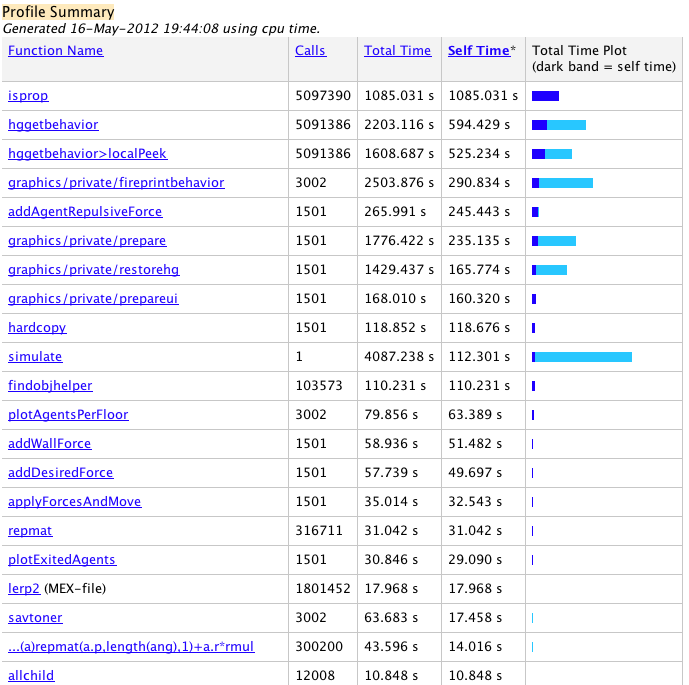
\includegraphics[width=0.9\textwidth]{./images/profiler.png}
\end{center}

We tried to optimize the code using the parallel for-loop parfor in matlab. In
the function applyForcesAndMove we replaced the for-loop over the agents with
parfor. We measured the time using an input with 200 agents on a 4 core machine
using 5 matlab workers. The result was that the parfor version was even slightly
slower than the serial version. The reason for this is how matlab implements
parfor: all the memory that is used by a worker must be sent to this worker.
Each agent must access the building floor image randomly and this creates a
large amount of memory that must be transferred to each worker, which leads to a
decreasing performance.
This is why we decided not to use parfor or any other parallelization in our
implementation.

\section{Simulation Results and Discussion}

\subsection{Expected Results}

We expect the stairs and the main building exit to be the bottlenecks. The amount of people in lower levels is increasing with time until a certain point, when most of the people have exited the building. Also we think that if the speed (velocity) of the people is higher (people are more in panic), jams at the exit will increase and people will mainly try to take the main exit instead of emergency exits.

\subsection{Simulation Results}

%TODO: add some plots, ...

\subsection{Discussion}


\section{Summary and Outlook}

In this section we would like to thank the MSSSM-Group from the ETH in Zurich, Switzerland directed by Karsten Donnay and Stefano Balietti for their engagement in the lecture "Modeling and Simulating Social Systems with MATLAB" during the Spring Semester 2012.


%TODO: Rückblick aufs projekt & Danksagung

\section{References}

\begin{thebibliography} {9}
	
	\bibitem{SFMPD} Helbling, Dirk - Molnar, Peter (1995): Social Force Model for Pedestrians Dynamics.
	\bibitem{AACIBF} Helbling, Dirk, Johansson, Anders (2006): Analytical Approach to Continuous and Intermittent Bottleneck Flows.
	\bibitem{ACPPD} Schadschneider, Andreas et al. (2002): CA Approach to Collective Phenomena in Pedestrian Dynamics.	
	\bibitem{DCD} Helbling, Dirk, Johansson, Anders (2007): Dynamics of crowd disasters: An empirical Study.
	\bibitem{SDFEP} Helbling, Dirk et al. (2000): Simulating dynamical features of escape panic.
	\bibitem{SPCD} Helbling, Dirk et al. (2005): Self-Organized Pedestrian Crowd Dynamics: Experiments, Simulations, and Design Solutions

\end{thebibliography}

% use \cite{SFMPD} for citation

\section{Appendix}

\subsection{Code}

%TODO: (Felix) Format of Code
\lstset{language=Matlab,breaklines=true}

\lstinputlisting[caption=simulate.m]{../code/simulate.m}
\lstinputlisting[caption=plotFloor.m]{../code/plotFloor.m}
\lstinputlisting[caption=plotExitedAgents.m]{../code/plotExitedAgents.m}
\lstinputlisting[caption=plotAgents.m]{../code/plotAgents.m}
\lstinputlisting[caption=loadConfig.m]{../code/loadConfig.m}
\lstinputlisting[caption=initWallForces.m]{../code/initWallForces.m}
\lstinputlisting[caption=initialize.m]{../code/initialize.m}
\lstinputlisting[caption=initEscapeRoutes.m]{../code/initEscapeRoutes.m}
\lstinputlisting[caption=initAgents.m]{../code/initAgents.m}
\lstinputlisting[caption=imageToMat.m]{../code/imageToMat.m}
\lstinputlisting[language=C,caption=getNormalizedGradient.c]{../code/getNormalizedGradient.c}
\lstinputlisting[language=C,caption=fastSweeping.c]{../code/fastSweeping.c}
\lstinputlisting[caption=checkForIntersection.m]{../code/checkForIntersection.m}
\lstinputlisting[caption=applyForcesAndMove.m]{../code/applyForcesAndMove.m}
\lstinputlisting[caption=addWallForce.m]{../code/addWallForce.m}
\lstinputlisting[caption=addDesiredForce.m]{../code/addDesiredForce.m}
\lstinputlisting[caption=addAgentRepulsiveForce.m]{../code/addAgentRepulsiveForce.m}

%TODO: Add all code-files

\end{document}  



 
